\chapter{Design and Development}
\label{chapter:designanddevelopment}

\section{Data source}

\subsection{CrimeBB}

Data source for current project is \textit{CrimeBB} \cite{crimeBB} database from Cambridge Cybercrime Centre. This database is made up of information collected from the main underground forums, through web scrapping. \\
Content of the database has been provided in the form of PostgreSQL dumps (.sql files). In order to make it possible to handle and query DB registries, these dump files have been loaded in a dockerized PostgreSQL database engine. \\
Steps needed for creating and Hydrating DB are described in project's source code \texttt{README.md} file. Files needed to do these steps are under \texttt{docker/postgres\_crimebb} folder.

\begin{figure}
	\centering
	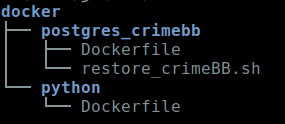
\includegraphics[width=0.4\textwidth]{figs/crimebb_tree.png}
	\caption{CrimeBB docker folder tree}
	\label{fig:crimebb_tree}
\end{figure}

\newpage

\subsection{Database structure}

Schema shown in image \ref{fig:crimebb_structure} describes how data models have been defined in it's tables, data field types and relations between them.

\begin{figure}[H]
	\centering
	\includegraphics[width=0.8\textwidth]{figs/crimebb.png}
	\caption{CrimeBB database structure}
	\label{fig:crimebb_structure}
\end{figure}

\noindent
\underline{NOTE}: \\
Schema shows relations between models, but provided DB data does not include foreign keys that ensure these relationships. That would be desirable in order to ensure data integrity.
\newpage

\section{Project Architecture}

\subsection{Overview}

All needed project components are self contained in a folder. It includes all needed \textit{Docker} and \textit{Docker-compose} stuff, \textit{Python} source code, generated datasets, \textit{Jupyter Workbook} ad so on ... \\
It is intended for allowing anyone to clone project's git repository and build up project in order to reproduce all results. For details on how to run it, see \texttt{README.md} in project root folder. \\
Just to prevent database content from being accidentally shared without permission, CrimeBB \texttt{.sql} dump files are not included in project folder. For the same reason, the container folder for the docker volume, from PostgreSQL, is also outside the project's root directory.

\subsection{Architecture}

Curent project source code architecture follows \textit{Hexagonal Architecture principles} (see figure \ref{fig:hexarch}), also known as \textit{Ports and Adapters}. This architecture was firstly described by Dr. Alistair Cockburn \cite{cockburn} and adopted by Steve Freeman, and Nat Pryce in their book \textit{Growing Object-Oriented Software Guided by Tests} \cite{growingoos}. \\
It is meant to be a flexible, changes ready way of structuring software projects. It is based in the \textit{Clean Code} principles, described by Robert C. Martin (Uncle Bob) in his well known \textit{The Clean Architecture} \cite{unclebob} article.
\newline
This architecture is divided in three main layers:
\begin{itemize}
    \item \textbf{Infrastructure}: The outer layer. Controllers and all I/O related stuff (DB access, file readers/writers, ...). Anything that can change by an "external" cause (not by your decision), is in this layer. It includes repositories specific implementation, known as \textit{adapters}. 
    \item \textbf{Application}: Use cases represented by application services. In essence, these are actions launched from outside, which aim to solve use cases typical of the business logic that this project intends to support.
    \item \textbf{Domain}: Inner layer. Business context and rules goes here, represented by models and domain services. Repository Interfaces, known as \textit{ports}, belongs to this layer.
\end{itemize}
\newpage

\begin{figure}[H]
	\centering
	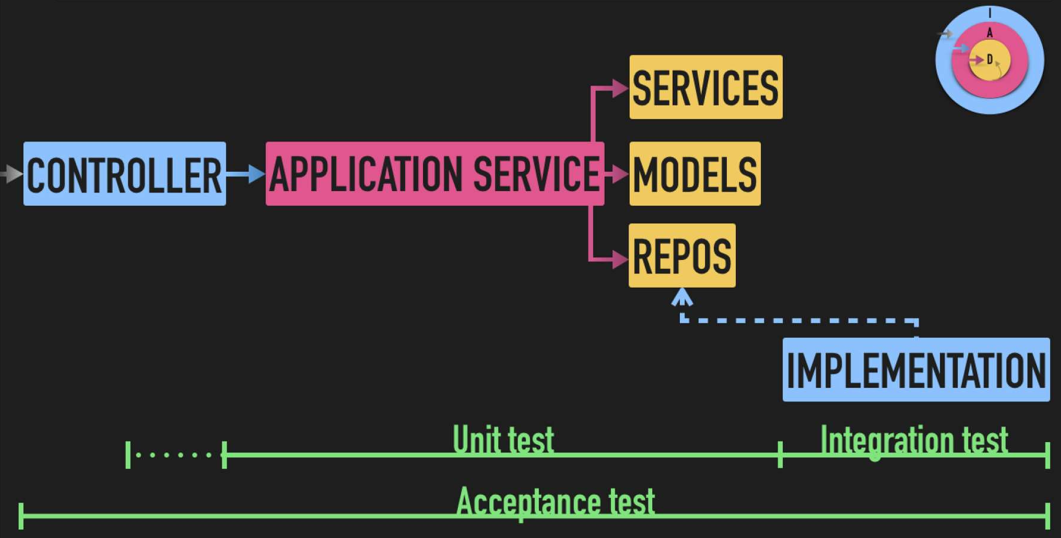
\includegraphics[width=0.8\textwidth]{figs/hex_arch_schema.png}
	\caption{Hexagonal Architecture}
	\label{fig:hexarch}
\end{figure}

This project has an important part of data exploration that makes it necessary to be able to change, in an agile way, the way to extract and process data. \\
Requirements could change along development process. According to that, main reasons for choosing this architecture are:
\begin{itemize}
    \item Layers distribution is intuitive. So it eases finding software component in the place that it is figured to be.
    \item Testing code is mandatory in order to build good quality software, reliable and easy to maintain. This architecture makes it easy to build software using \textit{TDD} (Test Driven Development) methodology.
    \item It allows to change the objectives, re-using as much code as possible, without the project structure ending up being a disaster.
\end{itemize}

\subsection{Testing}
In accordance with good practices widely accepted by the software developer community, Development has been done by following TDD (Test Driven Development) principles. TDD is now an established technique for delivering better software faster. TDD is based on a simple idea: writing tests for the code before writing the code itself. \\
For every layer, main component directories, contains a \texttt{tests/} folder with complete tests cases. Tests have been built with \texttt{unittest} Python library. \\
Running full tests battery is as easy as running the following command inside \texttt{python} docker container or within a Python virtual environment that meets \texttt{requirements.txt} packages:
\begin{verbatim}
    python -m unittest -v
\end{verbatim}

\section{Dataset generation helper software}
\label{sec:automaticprocess}

\textit{Ground truth} and \textit{full} datsets will contain \textit{HackForums} data. For this project, relevant data is placed in sub-forums under \textit{Market} section (the palce were services are supplied and demanded). \\
So, first step for building our datasets is to extract relevant data from Threads in these sub-forums. To do so, a Python tool has been built in order to connect to PostgreSQL DB and extract Threads and Posts from these subforums. \\
Once relevant information has been extracted from these Threads, DDoS related information is filtered and pre-annotated.

Resulting data is saved in a CSV dataset, that will be the seed of final datasets (see \autoref{sec:preannotate}). So, this pre-annotated datset,will be the starting point for the manual work necessary to prepare the \textit{supply} and \textit{demand} datasets that will be used to form the \textit{ground truth} and the \textit{full} datasets. \\
Both datasets, \textit{supply.csv} and \textit{demand.csv}, are the result of manual work. These datsets are then mixed and used for building \textit{ground truth} and \textit{full} (see \autoref{sec:builddatasets}). The former will be used for training and evaluating classification models and the latter is meant to be annotated by the selected model. That annotated full dataset will finally be used for data analysis in Jupyter Workbook.

\textbf{NOTE: } Manual work needed for creating \textit{supply.csv} and \textit{demand.csv} datasets is explained in \autoref{sec:datasetscreation}.

\newpage

\subsection{Generating pre-annotated dataset}
\label{sec:preannotate}

For generating pre-annotated dataset just execute Python tool entrypoint main file:
\begin{verbatim}
    python main.py annotate
\end{verbatim}
Resulting dataset CSV file is saved in project folder \texttt{datasets/ddos\_auto\_annotated\_dataset.csv} \\
The process can be summarized as shown in figure \ref{fig:preannotate}.

\begin{figure}[H]
	\centering
	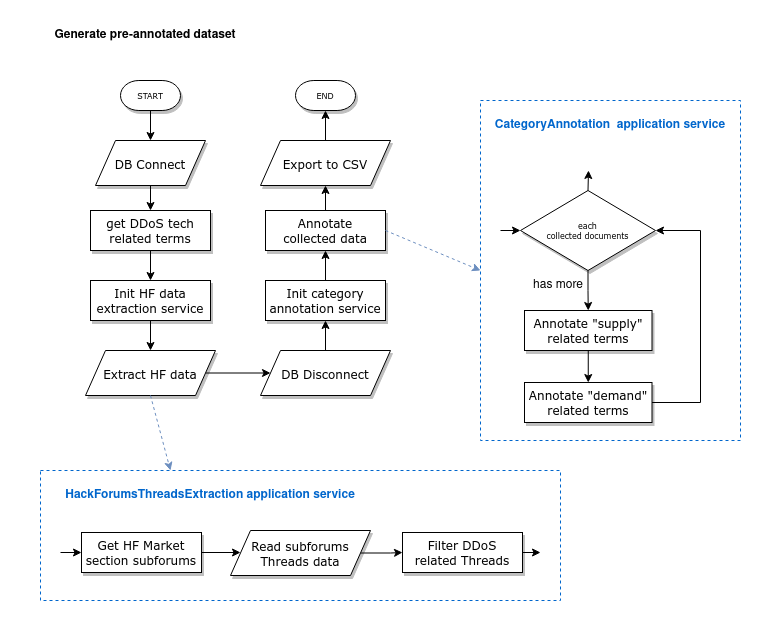
\includegraphics[width=1.0\textwidth]{figs/preannotate.png}
	\caption{Pre-annotate process}
	\label{fig:preannotate}
\end{figure}

\newpage

\subsection{Generating \textit{ground truth} and \textit{full} datasets}
\label{sec:builddatasets}

The result of manual work is \textit{supply.csv} and \textit{demand.csv} datasets. These datasets are then mixed to obtain \textit{ground truth} and \textit{full} datasets. To do that, Python tool is used as follows:
\begin{verbatim}
    python main.py generate_datasets
\end{verbatim}
In addition to the two above, two other datasets will be generated: \textit{market\_section\_posts\_count\_dataset.csv} and \textit{ddos\_posts\_count\_dataset.csv}. The former is a resume of HF market section posts count, grouped by month. The latter is the same but only DDoS related posts are included. These two datasets are intended to be used, later, in Jupyer Workbook. Process overview is shown in \ref{fig:generationprocess}

\begin{figure}[H]
	\centering
	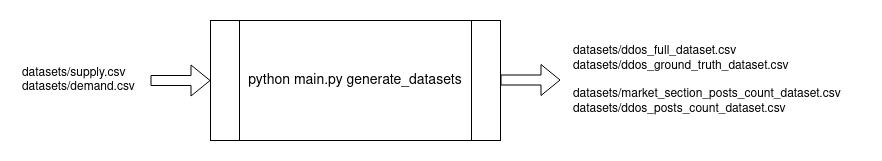
\includegraphics[width=0.8\textwidth]{figs/main.py.step2.png}
	\caption{Final datasets generation process}
	\label{fig:generationprocess}
\end{figure}

Figure \ref{fig:datasets_building} shows diagram flow on how all those four datasets are generated.

\begin{figure}[H]
	\centering
	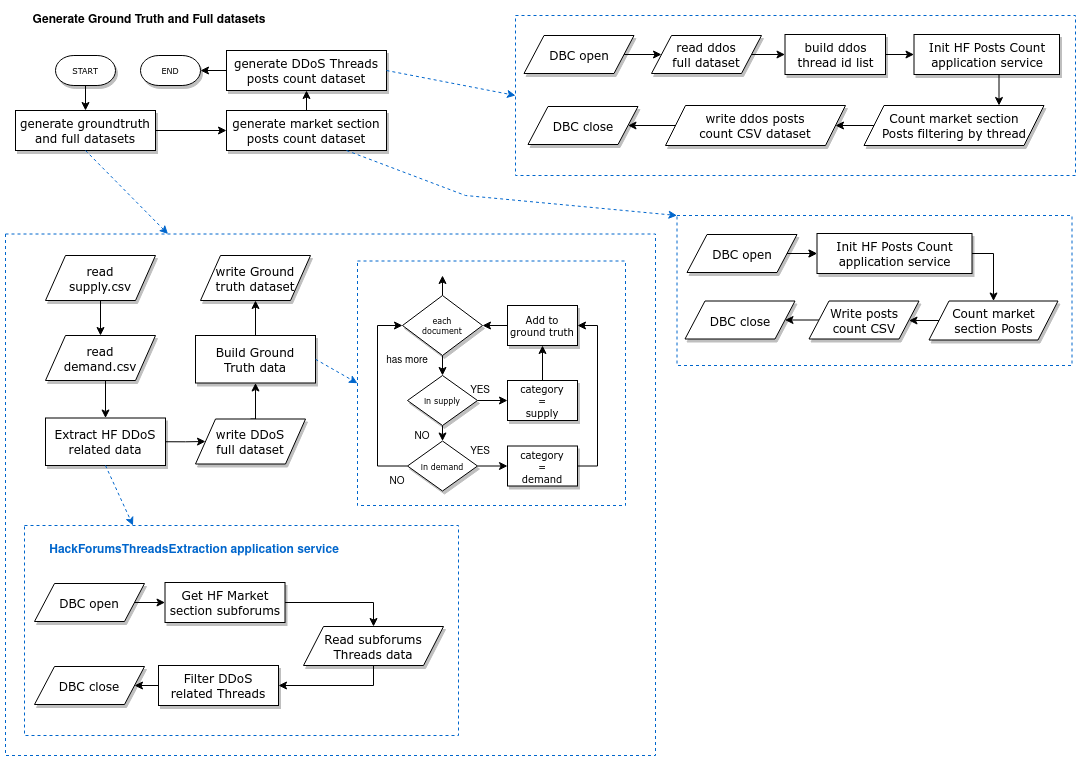
\includegraphics[width=1.0\textwidth]{figs/main.py_4_datasets.png}
	\caption{Final datasets generation detailed process}
	\label{fig:datasets_building}
\end{figure}

\section{Datasets creation process}
\label{sec:datasetscreation}

Datasets creation process consists in a mix of automated tasks and a lot of manual work. Automated processes have been covered in \autoref{sec:automaticprocess}. This section shows the full process.\\
Diagram \ref{fig:datasets_full_process} describes the workflow from when we generated the first pre-classified dataset, through manual refining and classification, to the construction of the final datasets.

\begin{figure}[H]
	\centering
	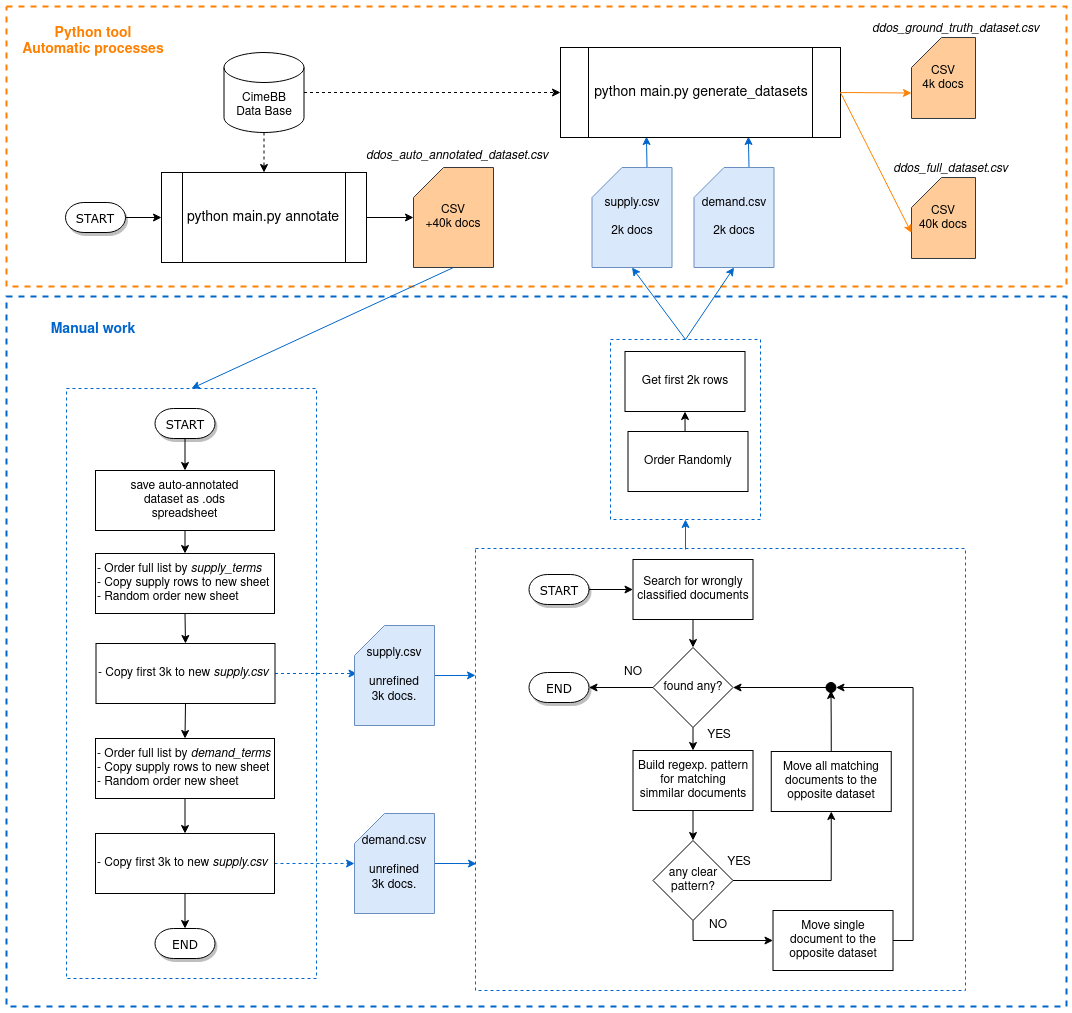
\includegraphics[width=1.0\textwidth]{figs/datasets_full_process.png}
	\caption{Final datasets generation detailed process}
	\label{fig:datasets_full_process}
\end{figure}

\section{Data analysis}
\label{sec:dataanalysis}

Final purpose of development phase is to analyse cimeBB DB data in order to know how \textit{Sale of access IoT devices} for DDoS is traded in underground forums.
Once annotated dataset and a full dataset have been built, data analysis tasks can be performed.\\
Jupyter Workbook has been selected as the tool for this final stage. It allows to write Python code and importing external libraries in order to load and analyse data and graph results. Despite data analysis and results obteined in Jupyter workbook are explained in chapter \ref{chapter:data_analysis_results}, this section describes main aspects of it.\\
Workbook sections are:
\begin{itemize}
    \item \textbf{Data source}: It loads datasets in pandas dataframes \cite{dataframe} and shows its structures.
    \item \textbf{Data pre-process}: Data clean, Tokenization and calculate \textit{tf and tf-idf} (Term Frequency times Inverse Document Frequency).
    \item \textbf{Model training}: Train some well known model types, commonly used in classification tasks (Linear Support Vector Classification, Stochastic Gradient Descent, K-nearest Neighbor, Multinomial Naïve Bayes).
    \item \textbf{Model evaluation}: Calculate \textit{accuracy}, \textit{precision}, \textit{recall} and \textit{F1 score}, and graph ROC curve in order to select best performing model.
    \item \textbf{Data Analysis}: In order to know how \textit{Sale of access IoT devices} has evolved in last years, we graph timeseries for main topics, segmenting by \textit{supply} and \textit{demand}. These main topics are: Supply \textit{vs} demand ratio, most used DD0S related tech terms, payment methods.
\end{itemize}
